%% -*- coding: utf-8-unix -*-

\chapter{課題に対するアプローチ}
\label{chap:approach}

\section{自動テストの基礎知識}
\label{sec:latedge-test-automation}

 % NetTester機能拡張検討
 % \url{https://drive.google.com/file/d/0B2eRR_JxYJA5TmhaeWItNF93Um8/}
 % ITHD技術交流会資料
 % \url{https://drive.google.com/drive/folders/0B2eRR_JxYJA5OFkzUFlveVlObWc}
 % ool意見交換会1019
 % \url{https://drive.google.com/drive/folders/0B2eRR_JxYJA5NHcxX0ZuTm9ZTEk}

  \subsection{自動テストの一般的な動向}
  \label{sec:popular-test-automation}

ソフトウェア開発においては、システム(アプリケーション)の自動ビルド・自動
デプロイ・自動テストなどがおこなわれ、特に近年では CI/CD や DevOps といっ
たかたちでノウハウやベストプラクティスの蓄積・共有・ツールや環境の整備な
どのとりくみをおこなうことが一般的になった。

また、クラウドサービスを背景に、アプリケーション(ソフトウェア)だけでなく
システム基盤についてもソフトウェアによる構築や制御が可能になってきた。ソ
フトウェアによってシステム基盤全体を制御するという考えかたは、IaC
(Infrastrucure as Code) や SDx(Software Defined Anything) /
SDI(Infrastructure) / SDDC(DataCenter) など様々なコンセプトで実現される
ようになってきている。

CI/CDやDevOpsなどの取り組みは、単なるソフトウェア開発の範囲だけでなく、
ソフトウェアによって制御可能な(クラウドサービスベースの)システム基盤を含
むシステム(あるいはサービス)全体でとりくまれるようになっている。こうした
取り組みでは、アプリケーションとシステム基盤全体の構築・運用を最適化し、
システムの利用者への価値提供 = サービス価値を最大化することが求められる。

  \subsection{「ふるまい」のテスト}
  \label{sec:behavior-test}

  % サービスのテストとは? →二重の円の図
  % なぜトップダウンにやるべきなのか
  % (無駄なテストをさける/DHHのはなし:高宮さんTremaday沖縄資料, TDD/BDDまわりの話)
  % \url{https://3.basecamp.com/3088280/buckets/867009/uploads/317155391}

\ref{sec:popular-test-automation}節で取り上げたように、CI/CDといった開発・
運用プロセスのとりくみがソフトウェア開発分野を中心におこなわれている。本
プロジェクトではそうした考えかたをシステム基盤(ネットワーク)の構築・運用
に適用していくことを考える。ネットワークのテストを自動化するにあたって、
ソフトウェアの自動テストなどで確立されたベストプラクティスやツールなどを
応用するかたちになることが効果的だと言える。そこで、本プロジェクトでは、
ネットワークをBDD(Behavior Driven Development)の考えかたをもとにテストす
ることを考えた。

BDDはTDDから派生した開発手法で、開発するソフトウェアに期待される「ふるま
い」に対するテストである~\cite{wikipedia-bdd}。BDDではソフトウェアに期待
される「ふるまい(Behavior)」、つまり、ソフトウェアの複数の機能を連結した
end-to-end でのインテグレーションテストを行なう
(\figref{fig:test-difference})。

\begin{figure}[h]
 \centering
 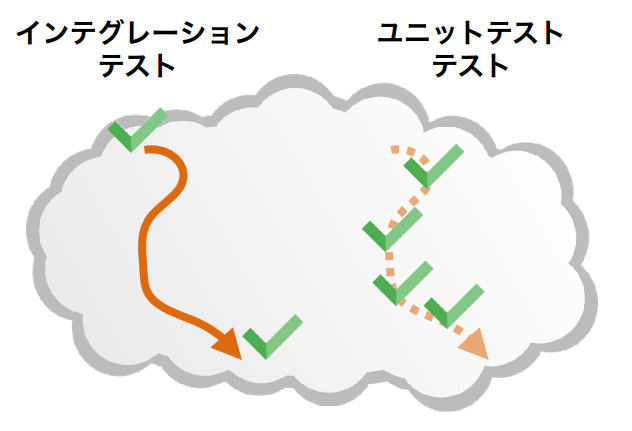
\includegraphics[scale=0.6]{img/test-difference.png}
 \caption{インテグレーションテストとユニットテスト}
 \label{fig:test-difference}
\end{figure}

仕様(spec)にもとづいたインテグレーションテストを最初におこなうようにする
ことで、以下のようなメリットがある。
\begin{itemize}
 \item テストの目的を明確にする
 \item 実際的なテストができる
 \item 無駄なテストをおこなわない
\end{itemize}

BDDでは、まずインテグレーションテスト(仕様上期待されるふるまい)について
のテストをおこない、問題があった場合に内部を詳細化したユニットテストに分
割して原因をきりわけるようにする(\figref{fig:bdd-cycle}\footnote{図引用:
Should TDD and BDD be used in conjunction? - Stack Overflow
\url{http://stackoverflow.com/questions/33746804/should-tdd-and-bdd-be-used-in-conjunction}})
。
% BDD test cycle の図をいれる
\begin{figure}[h]
 \centering
 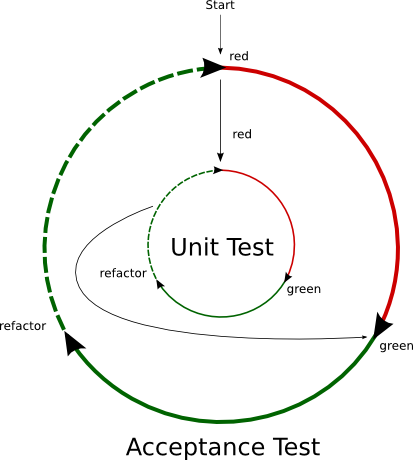
\includegraphics[scale=0.5]{img/bdd-cycle.png}
 \caption{BDDサイクル}
 \label{fig:bdd-cycle}
\end{figure}

インテグレーションテストがパスすれば詳細なテストを省略し、インテグレーショ
ンテストで失敗した場合にユニットテストを実施して原因の切り分け・修正をお
こなう。こうすることによって、不要なユニットテストの実装・実行にともなう
開発効率の低下を回避し、最終的にシステム(ソフトウェア)の利用者に対して価
値を提供しているか(期待される仕様を満たすか)どうかを基準にテストをおこな
う。インテグレーションテストでは、テスト対象とするシステム(ソフトウェア)
の最終的なふるまいをテストするため、仕様とテストシナリオがほぼ直接マッチ
する。したがって、BDDのテストシナリオを記述する作業は製品が満たすべき仕
様を具体的に定義したものとなる。

通常、テストコードは直接的に金銭的報酬を発生させるものではなく、開発にお
いてテストによる品質担保とテスト対象(プロダクト)とのバランスを適切に保つ
必要がある。ユニットテストなどの詳細化された機能単位のテストでは、個々の
機能としての動作は確認できるが、複数の機能を組合せ・連結して最終的にどの
ような動作をするか、というテストとの対応が結びつけにくい。こうした状況で
は、往々にして「ユニットテストをもれなく作成すること」「テストカバレッジ
を100\%にすること」が目的化されがちである。しかしもちろん、個々のユニッ
トテストがパスしても、最終的にテスト対象となる製品が(利用者が求める)仕様
を満たさなければ価値がない。BDDでは最終的に製品が満たすべき仕様に着目し、
テスト対象が実現すべき価値の観点で無駄なテストを減らすことを想定している。

 \section{理想像とプロジェクトのターゲット}
 \label{sec:desired-and-target}

 % 理想的にはどうなってほしいのか
 % ここではどこらへんをおとしどころにするか

  \subsection{テストしたいネットワークの「ふるまい」}
  % ネットワークの「ふるまい」とは何か?
  % 動的なテスト, 静的なテストとは何か?

\ref{sec:behavior-test}に示したとおり、本プロジェクトではBDDの考えかたに
そって、ネットワークの「ふるまい」をテストする。ネットワークのふるまいと
して、大きくいかの2点を考える。
\begin{itemize}
 \item 静的なふるまい
 \item 動的なふるまい
\end{itemize}

    \paragraph{静的なふるまい}
ネットワークが定常状態にあるときに、end-to-end でどのような通信ができる
か(end-to-endの通信試験: \figref{fig:test-static})。ネットワークにもとめ
られ最も基本的なる機能要求は、必要なノード間/アプリケーション間で通信が
できることである。静的なふるまいとして、ネットワークの状態がかわらない
(一定のトポロジ/一定の状態、例えば、通常利用していて特にイベントが発生し
ていない状況)ときに、アプリケーションレベルでの通信が実現できる(できない)こ
とを確認する。
% 図をいれる: net_tester/examples readme にいれたやつ。
\begin{figure}[h]
 \centering
 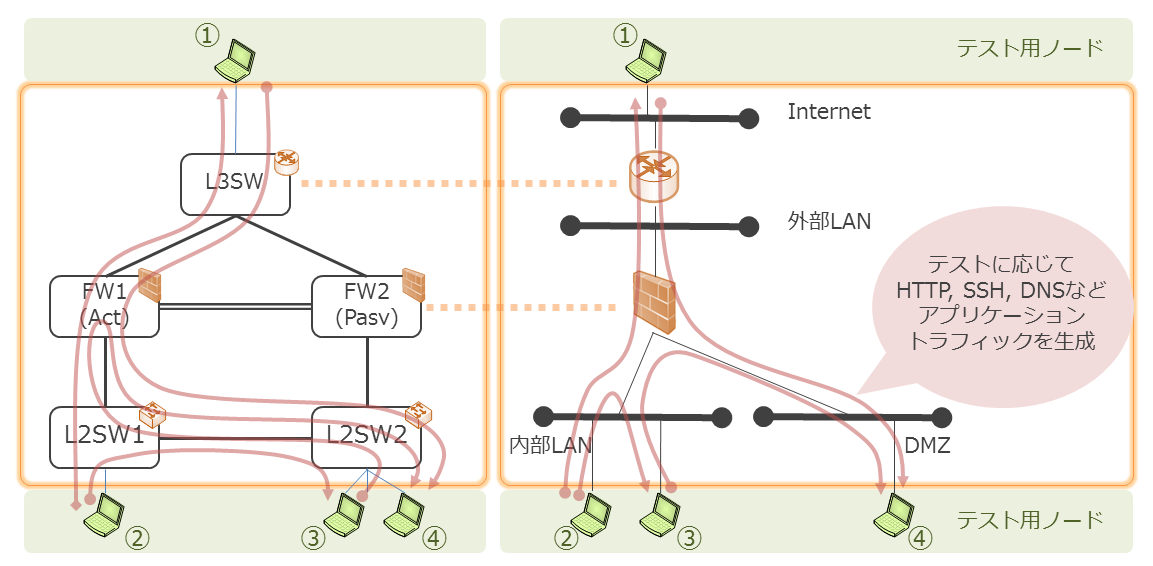
\includegraphics[scale=0.5]{img/test-static.png}
 \caption{ネットワークの静的なふるまいのテスト}
 \label{fig:test-static}
\end{figure}

このような通信試験においては、適切な場所(物理的・論理的な位置)にノードを
設置すること、なるべく実際的な(実際利用されたときに発生するトラフィック
にちかい)テストトラフィックを発生させることがポイントとなる。

    \paragraph{動的なふるまい}
ネットワークは、耐障害性・拡張性を保証するために、ネットワーク機器間で相
互に制御情報を交換し、動的にネットワーク全体のトラフィック制御をおこなう。
\footnote{たとえば、ある機器に障害が発生し、その機器でトラフィックが中継
できないと(周囲の機器が)判断した場合、その機器を中継しないようにネットワー
クのトラフィック転送ルールが再構成される。}こうしたネットワーク自身の状
態変化がともなう状況を動的なふるまい、ととらえる。

定常状態にあったネットワークで、イベントに対して動的なふるまいが発生する
と、ネットワークの状態\footnote{トポロジ、あるいはNW機器の持つ状態(経路
情報, Acitve/Standbyなどの状態など)}が別の定常状態へと変化する。状態変化
の過程では、利用しているネットワーク機器の機能や仕様により、テストトラ
フィックパスが変更され、一時的に転送が中断/再開したりする。動的なふるま
いのテストは、こうした状態遷移中の通信状況を確認するものである
(\figref{fig:test-dynamic})。
% 図をいれる: net_tester/examples readme にいれたやつ。
\begin{figure}[h]
 \centering
 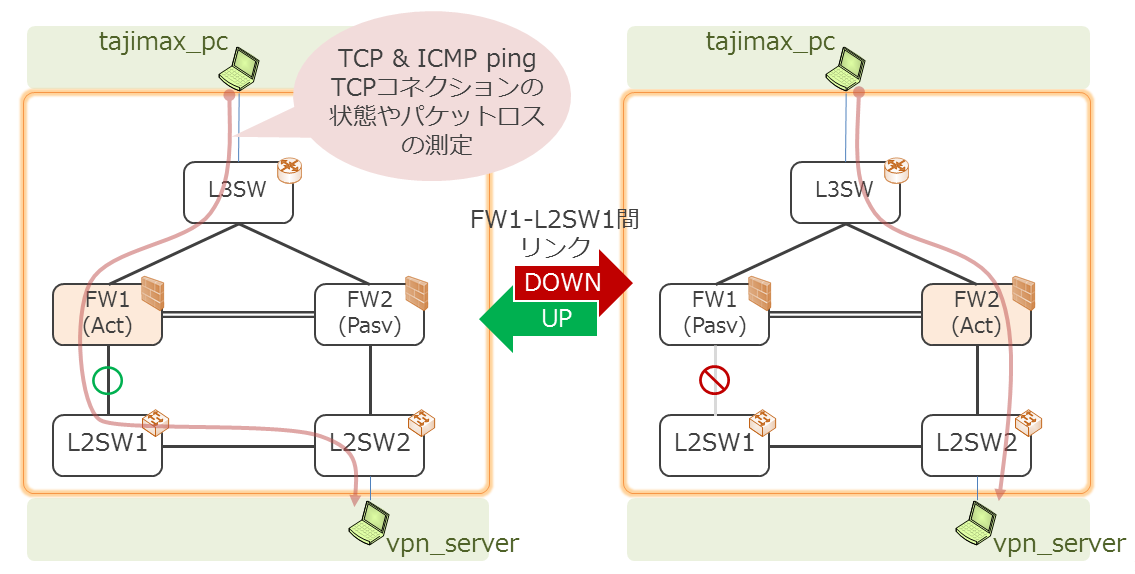
\includegraphics[scale=0.5]{img/test-dynamic.png}
 \caption{ネットワークの動的なふるまいのテスト}
 \label{fig:test-dynamic}
\end{figure}

動的なふるまいのテストでは、テスト対象ネットワークでの状態変化イベントの
発生、イベントをまたいだテストトラフィックの生成や通信状況の判断がポイン
トとなる。

  \subsection{ネットワークの自動テストと運用プロセス}
  \label{sec:network-test-and-process}

  % 既存の(ソフトウェア開発の)ツールや方法論が応用できること
  % だれに対して、どのようなメリットを提供するか?

\ref{chap:problem-setting}章で解説したように、現状ネットワークのテストは
人手によるところが多く、それがボトルネックになって網羅性やスケール性が低
い。ここでは、もし仮に、現状人手に頼らざるをえないネットワークの操作が機
械的に・自動実行できるとしたらどのような構築・運用プロセスをとることがで
きるかについて検討する。

ソフトウェアによってネットワークの操作が自由にできる(操作の自動化ができ
る)と仮定した場合、ネットワークに対する構築や運用についても、ソフトウェ
ア開発でおこなわれているベストプラクティスやノウハウがそのまま応用できる
形となることが理想的だと考える。これによって、
\figref{fig:desired-cicd-process}のようなかたちでシステムの自動構成・自
動テスト、本番システムデプロイというCI/CDプロセスを実現させることができ
る。
\begin{itemize}
 \item システム(ネットワーク)で実現すべき要求を定義する
 \item 要求をコード化する
       \begin{itemize}
        \item 要求を実現するためのコード(ネットワーク設計/実装)
        \item 要求を確認するためのコード(ネットワークが満たすべき「ふる
              まい」: ネットワーク上で実現されるべき通信やネットワーク自
              身の動作)
       \end{itemize}
 \item 検証環境で自動構築・自動テストをおこなう
       \begin{itemize}
        \item テストが失敗したら原因を分析し、コードを修正・再テストをおこなう
       \end{itemize}
 \item 自動テストがすべてパスしたら本番環境へのデプロイをおこなう
\end{itemize}

% 図をいれる: ぐるぐるまわす図
\begin{figure}[h]
 \centering
 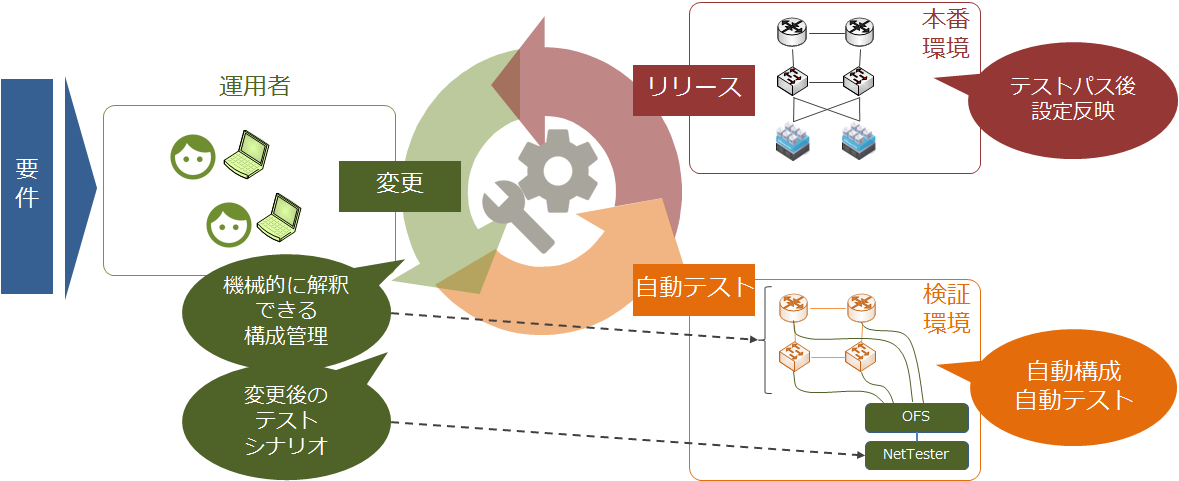
\includegraphics[scale=0.5]{img/desired-cicd-process.png}
 \caption{ネットワークのCI/CDプロセス}
 \label{fig:desired-cicd-process}
\end{figure}

ネットワーク(に限らずシステム基盤)では、ハードウェア製品を多様するため本
番環境とまったく同等の検証環境を整備することは通常難しい。しかし、性能面・
拡張性の問題などをある程度スコープ外とすることで、仮想アプライアンスなど
を利用して小規模でも機能的には同等の環境を整備することができるようになっ
ている。このように、仮想化技術の応用をふくめて、機器/環境をソフトウェア
で制御できる範囲がひろがり、自動化されるにともない、まず自動構築のための
技術・ツール・ノウハウが発展しつつある。

本プロジェクトは、そこに(ネットワークの)テストという構成要素を補い、上記
のようなシステム基盤のCI/CD実現を促進させることを狙っている。

 \section{ネットワークテストシステムの検討}
 \label{sec:discuss-network-test}

 % OOD発表資料p.4-5 「6個の構成要素」の話。ここでターゲットにするものは何か?
 % ネットワークの操作を自動化するために必要なことは?
 % テストの自動化のためにどういった機能コンポーネントが必要か?

ネットワークのテストを自動化するにあたって、現状手作業でおこなっている操
作を機械的に実行できるようにしなければならない。本プロジェクトでは、ネッ
トワークのテストのために必要な操作を
\figref{fig:features-of-network-testing}・\tabref{tab:test-functions}の
ように分類している。

\begin{figure}[h]
 \centering
 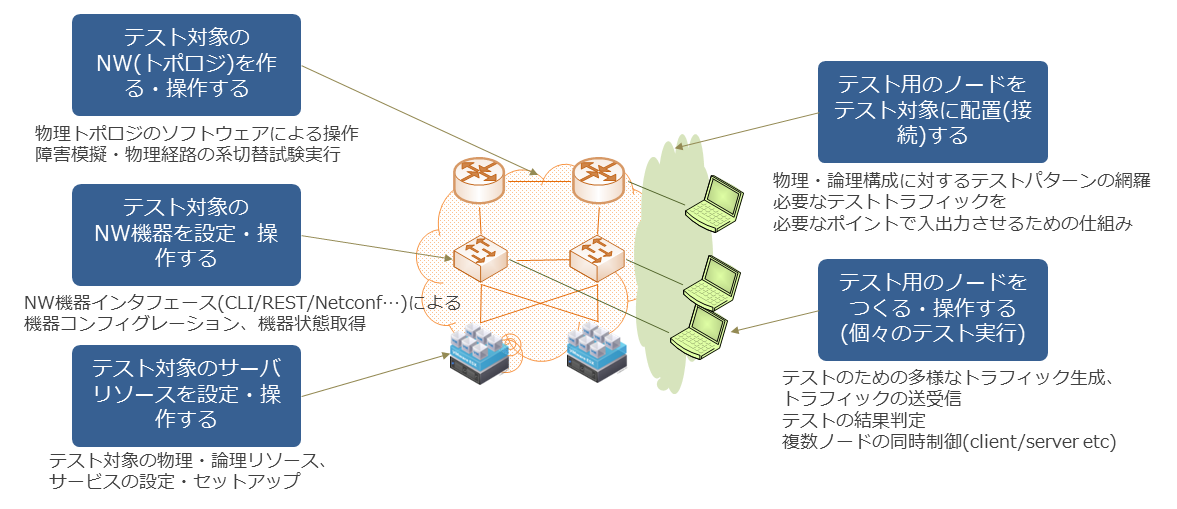
\includegraphics[scale=0.5]{img/features-of-network-testing.png}
 \caption{ネットワークテスト自動化のための機能要素}
 \label{fig:features-of-network-testing}
\end{figure}

\begin{table}[h]
 \caption{NWテスト自動化に必要な機能要素}
 \label{tab:test-functions}
 \begin{center}
  \begin{tabular}[t]{l|l|p{25em}}
   \hline
   No. & 要素 & 役割 \\ \hline
   \hline
   1 & NW機器を設定・操作する & テスト対象ネットワークにあるNW機器の設定を変更する \\ \hline
   2 & サーバリソースを設定・操作する & テスト対象ネットワークにある物理サーバ・仮想サーバのリソース操作などをおこなう \\ \hline
   3 & トポロジを操作する & テスト対象ネットワークのトポロジをソフトウェアによって操作する \\ \hline
   4 & テスト用ノードを配置する & テスト用のノードを生成し、テスト対象ネットワークの指定した箇所に配置(接続)する \\ \hline
   5 &テスト用ノードを操作する & テスト用のノードを操作し、テストトラフィックの生成をおこなう\\ \hline
  \end{tabular}
 \end{center}
\end{table}

    \paragraph{テスト対象NW内ノード操作}
\tabref{tab:test-functions} No.1-2 はテスト対象ネットワークを構成する機
器(ハイパーバイザなど仮想化基盤管理・操作を含む)である。こうした機器操作
のための技術・ツールなどは既に多数存在しているため、本プロジェクトではこ
こには注力しない。(既存の技術やツールを応用する。)

    \paragraph{トポロジ操作}
\tabref{tab:test-functions} No.3 はテスト対象ネットワークのトポロジ(物理
結線を含む)の操作である。障害試験(リンクダウンなど)や環境の構成拡張・縮
小(ノードの追加・削除などトポロジ変更)といった、ネットワークトポロジその
ものの変更が発生する際のネットワークのふるまいをテストするために必要とな
る。

\ref{sec:difficulty} で示したように、特に物理構成要素の操作は自動化がむ
ずかしい。\lopjc では、OpenFlow スイッチを応用したテスト対象ネットワーク
の物理トポロジ構成・操作についての実証実験を行なった。本プロジェクトでは
そこで実証した技術を応用してテスト対象ネットワークの物理トポロジ操作をお
こなう。

    \paragraph{テスト用ノード操作}
\tabref{tab:test-functions} No.4-5 はテスト用ノードの操作である。一般的
に、ネットワークのテストではテスト用のトラフィックの生成・受信をおこなう
ことによって、テスト対象ネットワークが問題なく動作しているかどうかを確認
する。テストトラフィックの送受信はテスト対象ネットワークを構成する機器
(NW機器やサーバ)を利用場合もあるが、ログ取得やテスト用ツール準備などの都
合から、何らかのテスト用ノード(PCなど)を別途用意することが多い
\footnote{特に新規構築の場合は、サーバ等テスト対象とするノードが利用でき
ない(存在しない)状態でネットワークのテストをおこなうこともある。}。こう
したテスト用ノードを利用したテストには以下のような問題がある。
\begin{itemize}
 \item テスト用ノード(機器台数)の上限
 \item テスト用ノードを操作する人(担当者人数)の上限
 \item 分散作業によるテスト全体での状況把握の難しさ
 \item テスト用ノードのセットアップ(IPなど)の手間
 \item テスト用ノードの配置(テスト対象NWへの接続)の手間
\end{itemize}

トポロジ操作同様に、\lopjc では、Linux Namespace を利用したテスト用ノー
ドの生成・集中制御とOpenFlow スイッチを応用したテスト用ノード配置につい
ての実証実験を行なった。本プロジェクトではそこで実証した技術を応用して、
より実用的なテストユースケース(テストシナリオ)の実現をおこなう。

 \section{基本的なアイディア}
 \label{sec:basic-tester-idea}

  % このプロジェクトでは、
  % 「ネットワークテストシステム」としてどういったシステムを作ろうとしたのか?
  % NetTester の基本的なアイディアというか、
  % そもそものパッチパネルベースにテストをやるっていう話

  % https://drive.google.com/file/d/0B2eRR_JxYJA5TmhaeWItNF93Um8/view
  % にある「もうちょっと一般化」くらいの粒度でいれてもいいかもしれない。

\ref{sec:discuss-network-test}節でネットワークのテスト自動化のために必要
な機能要素について解説したが、それらをもとにネットワーク「テスタ」に求め
られる機能要求について解説する。要求については \lopjtech も参照のこと。

ネットワークのテスト自動化では、従来手作業でおこなっていたのと同等の操作
を、ソフトウェアにより自動的かつプログラマブルに実現したい。そのために、
テスト対象ネットワークの物理トポロジを、テストシナリオに応じて動的に再構
成したり、テスト用のノードを動的に接続したりする
(\figref{fig:basic-idea})。そこで、様々なノード間をつなぎ合わせる機能を
準備する(\tabref{tab:test-functions} No.3-4)。

% patch model の基本的な概念図をいれる
% net-tester readme にある最初の図くらいのやつでよい。
\begin{figure}[h]
 \centering
 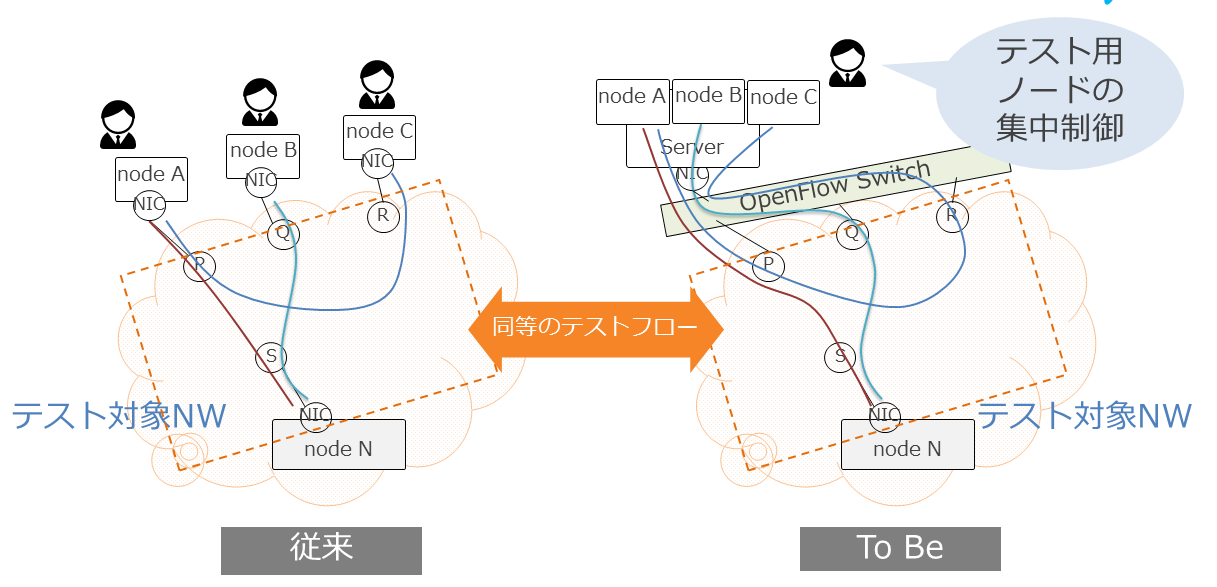
\includegraphics[scale=0.5]{img/basic-idea.png}
 \caption{テスターの基本アイディア}
 \label{fig:basic-idea}
\end{figure}

\lopjc では、安価かつトラフィック制御を自分で操作(プログラミング)可能な
OpenFlowスイッチを利用して、物理配線操作をするパッチパネルと同等のものを
実現し(\figref{fig:poc-l1patchpj}: \tabref{tab:test-functions}参照)、簡
単なテストユースケースのもとで有効性を確認した。

\begin{figure}[h]
 \centering
 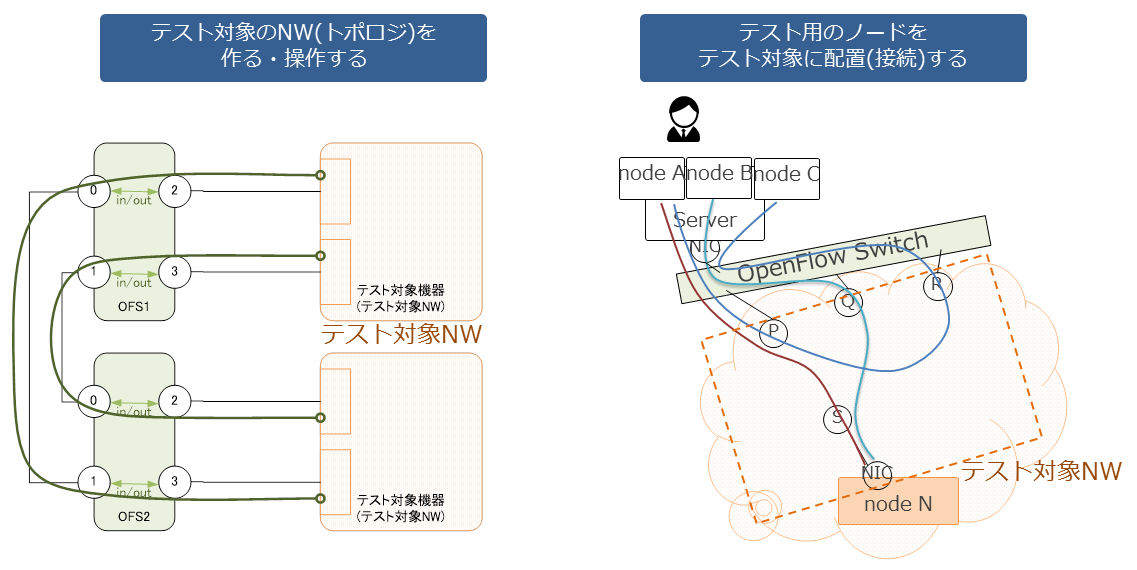
\includegraphics[scale=0.5]{img/poc-l1patchpj.png}
 \caption{\lopj PoCで実装・実証した機能要素}
 \label{fig:poc-l1patchpj}
\end{figure}


   % 「テスタ」に求められることは何か?
   % "patch panel" model – NetTester
   % \url{https://3.basecamp.com/3088280/buckets/867009/documents/208275139}
   % いるか??

 本プロジェクトは、\lopj の結果をもとに、NetTester~\cite{nettester} とい
 うテストツールを開発した。NetTester について
 は~\ref{chap:nettester-design}章で解説する。また、NetTesterをつかったネッ
 トワークテストのユースケース実証については~\ref{chap:poc}章で解説する。


%%% Local Variables:
%%% mode: yatex
%%% TeX-master: "main.tex"
%%% End:
